\prob
{
    Let $G$ be a connected plane graph.
    \begin{enumerate}[label=(\roman*)]
        \item Use matroid duality to show that $G$ satisfies Euler's polyhedron formula,
                \begin{align}
                        |V(G)| - |E(G)| + |F(G)| = 2,
                \end{align}
                where $F(G)$ is the set of faces of $G$.
        \item Prove that if $G$ is simple and $|V(G)| \geq 3$ then
                \begin{align}
                    |E(G)| \leq 3|V(G)| - 6.
                \end{align}
                
        \item Characterize the graphs for which equality is attained in (ii).
        
        \item Show that if $G$ is simple, then it has a vertex of degree at most five.
        
        \item Give an example of a simple plane graph in which every vertex has degree five.
    \end{enumerate}
}
\begin{proof}
    \begin{enumerate}[label=(\roman*)]
        \item
            We know that $|F(G)| = |V(G*)|$ that $r(M(G)) = |V(G)| - 1$, 
            that $r(M(G*)) = |V(G*)| - 1$, and that $|E(G)| = r(M(G)) + r(M(G*))$.\pn
            
            Then
            \begin{align}
                    |E(G)|  &=  r(M(G)) + r(M(G*))          \\
                            &=  |V(G)| - 1 + |V(G*)| - 1    \\
                            &=  |V(G)| + |V(G*)| - 2        \\
                            &=  |V(G)| + |F(G)| - 2        \\
            \end{align}
            
            And we are done.
        \item
            Given that $G$ is plane, then each face must have at least 3 edges.
            Then $3|F(G)| \leq 2|E(G)|$. From the equality from above
            \begin{align}
                    3|E(G)| + 6 &=      3|V(G)| + 3|F(G)|
                                &\leq   3|V(G)| + 2|E(G)|
            \end{align}
            
            Which can be rewriten as $|E(G)| \leq 3|V(G)| - 6$.
            
        \item
            If $G$ is such that all the minimum cycles (cycles whose vertex are not contained in bigger cycles) are 
            triangles. This means that any representation of $G$ is a triangulation. That is, every face is a triangle.\pn
            
            If every face is a triangle then $\frac{3}{2} |F(G)| = |E(G)|$ and then 
            \begin{align}
                   2                    &=  |V(G)| - |E(G)| + |F(G)|                \\
                   2                    &=  |V(G)| - |E(G)| + \frac{2}{3} |E(G)|    \\
                   2                    &=  |V(G)| - \frac{1}{3} |E(G)|             \\
                   \frac{1}{3} |E(G)|   &=  |V(G)| - 2                              \\
                   |E(G)|               &=  3|V(G)| - 6.                             
            \end{align}
            
            Now suppose that $G$ is not a triangulation, in any representation there will be at least one face that is
            not a triangle and then such face has at least a pair of vertices that are not adjacent. We can draw a new edge
            between such pair of vertices such that the resulting graph is also plane. Given the inequality from above and
            this new graph, $E(G) + 1 \leq 3|V(G)| - 6$, which means that $E(G) < 3|V(G)| - 6$.\pn
            
        \item
            If every vertex has degree at least $6$, given that $|E(G)| = \frac{\sum_{v \in V(G)} \delta(v)}{2}$, then
            \begin{align}
                |E(G)|      &=      \frac{\sum_{v \in V(G)} \delta(v)}{2}     \\
                            &\geq   \frac{6 |V(G)|}{2}                        \\                        
                            &\geq   3 |V(G)|                                  \\                        
            \end{align}
            
            Which means that $|E(G)| \geq 3 |V(G)| > 3 |V(G)| - 6$, contradictint the inequality form above.\pn
            
            
        \item
            The following graph meets the conditions.\pn
            \begin{center}
                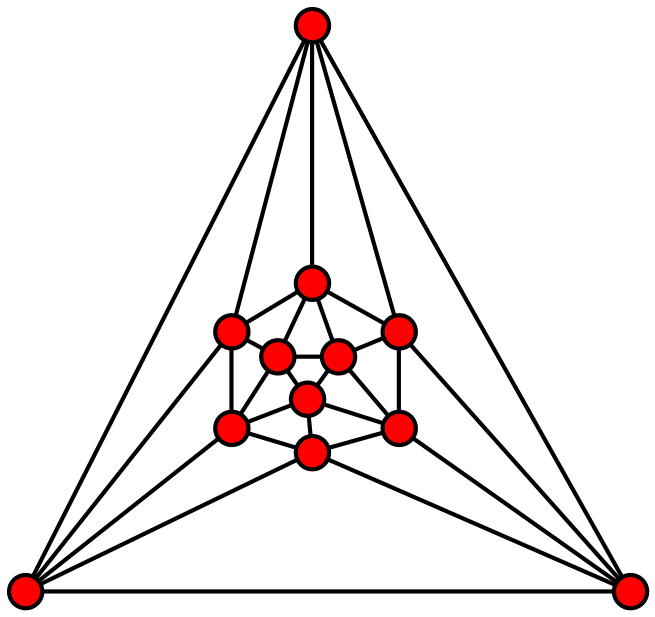
\includegraphics[width=4cm]{Test3/Problem4/Icosahedron_graph.png}
            \end{center}\pn            
    \end{enumerate}    
\end{proof}